\chapter[DNA, Chromosomes, and Genomes]{DNA, Chromosomes, \protect\\and Genomes}\labch{re}
The documents of biology, chemistry and other disciplines are characterized by more legends and noun explanations, and less formulas. Here we have created an command \Package{sidebysidecaption} to freely adjust the size of legends and figures.We use a portion of Chapter 4 of \citetitle{thecell}\sidecite{thecell}
 for our template presentation.



\section{The Structure of DNA Provides a mechanism for Heredity}\labsec{structure}

The discovery of the structure of DNA immediately suggested answers to the two
most fundamental questions about heredity. First, how could the information to
specify an organism be carried in a chemical form? And second, how could this
information be duplicated and copied from generation to generation?

The answer to the frst question came from the realization that DNA is a linear
polymer of four different kinds of monomer, strung out in a defned sequence like
the letters of a document written in an alphabetic script.

The answer to the second question came from the double-stranded nature of
the structure: because each strand of DNA contains a sequence of nucleotides
that is exactly complementary to the nucleotide sequence of its partner strand,
each strand can act as a \key{template}, or mold, for the synthesis of a new complementary strand. In other words, if we designate the two DNA strands as S and Sʹ, strand 

\begin{fullpage}

	\sidebysidecaption{0.5\linewidth}{0.45\linewidth}{%
		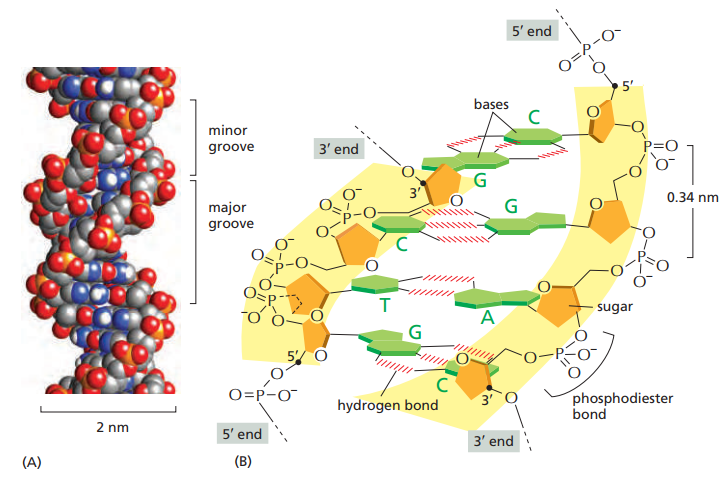
\includegraphics[width=1\linewidth]{img/double_helix.png}%
	}{%
	\captionof{figure}{The DNA double helix.
    (A) A space-flling model of 1.5 turns of
    the DNA double helix. Each turn of DNA is
    made up of 10.4 nucleotide pairs, and the
    center-to-center distance between adjacent
    nucleotide pairs is 0.34 nm. The coiling of
    the two strands around each other creates
    two grooves in the double helix: the wider
    groove is called the major groove, and the
    smaller the minor groove, as indicated.
    (b) A short section of the double helix
    viewed from its side, showing four base
    pairs. The nucleotides are linked together
    covalently by phosphodiester bonds that
    join the 3ʹ-hydroxyl (–OH) group of one
    sugar to the 5ʹ-hydroxyl group of the next
    sugar. Thus, each polynucleotide strand
    has a chemical polarity; that is, its two
    ends are chemically different. The 5ʹ end
    of the DNA polymer is by convention often
    illustrated carrying a phosphate group,
    while the 3ʹ end is shown with a hydroxyl}
    }
\end{fullpage}

S can serve as a template for making a new strand Sʹ, while strand Sʹ can serve as a
template for making a new strand S (\vreffig{template}). Thus, the genetic information in
DNA can be 
accurately copied by the beautifully simple process in which strand
S separates from strand Sʹ, and each separated strand then serves as a template
for the production of a new complementary partner strand that is identical to its
former partner.

\begin{fullpage}

	\sidebysidecaption{0.5\linewidth}{0.45\linewidth}{%
		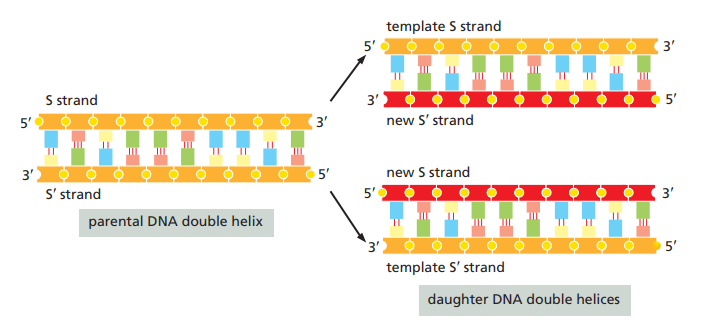
\includegraphics[width=1\linewidth]{img/template.png}%
        \labfig{template}}{%
	\captionof{figure}{DNA as a template for its
    own duplication. because the nucleotide
    A successfully pairs only with T, and g
    pairs with C, each strand of DNA can act
    as a template to specify the sequence of
    nucleotides in its complementary strand.
    In this way, double-helical DNA can be
    copied precisely, with each parental DNA
    helix producing two identical daughter DNA
    helices.}
    }
    
\end{fullpage}

The ability of each strand of a DNA molecule to act as a template for producing
a complementary strand enables a cell to copy, or replicate, its genome before
passing it on to its descendants. We shall describe the elegant machinery that the
cell uses to perform this task in Chapter 5.

Organisms differ from one another because their respective DNA molecules
have different nucleotide sequences and, consequently, carry different biological
messages. But how is the nucleotide alphabet used to make messages, and what do they spell out?

As discussed above, it was known well before the structure of DNA was determined that genes contain the instructions for producing proteins. If genes are made of DNA, the DNA must therefore somehow encode proteins (\vreffig{relation})\marginpar{
    \centering
    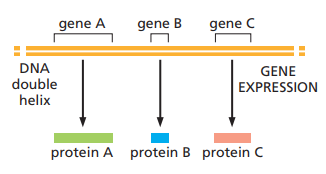
\includegraphics[width=0.4\textwidth]{img/relation.png}
    \captionof{figure}{The relationship between
    genetic information carried in DNA and
    proteins.}\labfig{relation}}.

As discussed in Chapter 3, the properties of a protein, which are responsible for its
biological function, are determined by its three-dimensional structure. Tis structure is determined in turn by the linear sequence of the amino acids of which it is
composed. The linear sequence of nucleotides in a gene must therefore somehow
spell out the linear sequence of amino acids in a protein. The exact correspondence between the four-letter nucleotide alphabet of DNA and the twenty-letter
amino acid alphabet of proteins—the genetic code—is not at all obvious from the
DNA structure, and it took over a decade after the discovery of the double helix
before it was worked out. In Chapter 6, we will describe this code in detail in the
course of elaborating the process of gene expression, through which a cell converts
the nucleotide sequence of a gene frst into the nucleotide sequence of an RNA
molecule, and then into the amino acid sequence of a protein.

